\chapter{图像及其数学与物理背景}
\section{概述}
在这里我们并不介绍所有必须的数学和物理基础,%
详细的内容请参看对应的物理和数学书籍。

\subsection{线性}
\textbf{\color{magenta}线性}这一概念将在本书中频繁出现:%
这与\textbf{\color{magenta}矢量空间}有关,%
其中常用矩阵代数。%
线性也与是矢量空间的更一般元素有关,%
比如,函数。%
在线性代数中\textbf{\color{magenta}线性组合}是一个关键概念,%
允许矢量空间的一个元素可以表示为已有元素与系数乘积的和。%
两个矢量$x,y$的一般线性组合可以写成$ax+by$,其中$a$和$b$是标量。%

考虑两个线性空间的映射$L$。%
如果$L(x,y)=L(x)+L(y)$,%
则称为加性的,%
如果对于任意的标量$a$有$L(ax)=aL(x)$,%
则称为单一性的。%
从实际角度看,这意味着输入的和产生各自输出的和。%
这一性质也称为\textbf{\color{magenta}叠加原理}。%
如果$L$是加性的且是单一性的,%
则称该映射是线性的。%
等价的,对于任意的矢量$x,y$和标量$a,b$,%
线性映射满足$L(ax+by)=aL(x)+aL(y)$,%
即它保持线性组合。

\subsection{狄拉克分布和卷积}
理想的冲击是一个重要的输入信号,%
图像平面上的理想冲击是用\textbf{\color{magenta}狄拉克分布}定义的,%
$\delta(x,y)$
\begin{equation}
  \int_{-\infty}^{\infty}\int_{-\infty}^{\infty}\delta(x,y)dxdy = 1
\end{equation}
且对于所有的$x,y\neq0$,有$\delta(x,y)=0$。%
狄拉克函数具有的筛选性
\begin{equation}
  \int_{-\infty}^{\infty}f(x,y)\delta(x-\lambda,y-\mu)dxdy = f(\lambda,\mu)
\end{equation}
它提供了函数$f(x,y)$在点$\lambda,\mu$处的值。%
该筛选公式可以用来描述连续图像函数$f(x,y)$的采样过程。%
我们可以将图像函数表示成覆盖整个图像平面的位于各点$(a,b)$的狄拉克
脉冲的线性组合,%
采样由图像函数$f(x,y)$加权,%
\begin{equation}
  \int_{\infty}^{\infty}\int_{-\infty}^{\infty}f(a,b)\delta(a-x,b-y)dady = f(x,y)
\end{equation}

\textbf{\color{magenta}卷积}在图像分析的方法中是一个重要的运算。%
卷积是一个积分,反映一个函数$f(t)$在另一函数$h(t)$移动时所重叠的量。%
函数$f$和$h$的在有限域$[0,t]$上的1D卷积$f*h$由下式给出:
\begin{equation}
  (f*h)(t) = \int_{0}^{t}f(\tau)h(t-\tau)d\tau
\end{equation}

为了准确起见,卷积积分的上下限是$(-\infty,\infty)$。%
这里可以限定在$[0,t]$区间,%
原因是我们假设负坐标部分的值为零。%
\begin{equation}
  (f*h)(t) = \int_{0}^{t}f(\tau)h(t-\tau)d\tau = \int_{-\infty}^{\infty}f(t-\tau)h(\tau)d\tau
\end{equation}
设$f,g,h$为函数,%
$a$是一个常数。%
则卷积具有如下的性质:
\begin{gather}
  f*h = h*f \\
  f*(g*h) = (f*g)*h\\
  f*(g+h) = (f*g) + (f*h)\\
  a(f*g) = (a f)*g = f*(a g)
\end{gather}
对卷积进行微分有
\begin{equation}
  \frac{d}{dx}(f*h) = \frac{df}{dx}*h = f*\frac{dh}{dx}
\end{equation}

卷积可以推广到更高维。%
2D函数$f$和$h$的卷积$g$记为$f*h$,%
通过积分定义为
\begin{equation}
  \begin{split}
    (f*h)(x,y) &= \int_{-\infty}^{\infty}\int_{-\infty}^{\infty}f(a,b)h(x-a,y-b)dadb\\
    &= \int_{-\infty}^{\infty}\int_{-\infty}^{\infty}f(x-a,y-b)h(a,b)dadb\\
    &= (h*f)(x,y)
  \end{split}
\end{equation}
在数字图像分析中,%
\textbf{\color{magenta}离散卷积}用求和来表达,%
而不是积分。%
数字图像在图像平面上有有限的定义域。%
但是,有限的定义域并不妨碍我们使用卷积,%
因为在图像定义域外它们的结果是零。%

线性操作中输出图像像素$g(x,y)$的计算结果是输入图像像素$f(x,y)$的一个局部邻域$\mathcal{O}$的亮度的线性组合。%
邻域$\mathcal{O}$中像素的贡献用系数$h$进行加权:
\begin{equation}
  f(i,j) = \sum_{(m,n)\in\mathcal{O}}h(i-m,j-n)g(m,n)
\end{equation}
上式与以$h$为核的离散卷积等价,%
称$h$为\textbf{\color{magenta}卷积掩膜}。%
一般使用具有为奇数的行和列的矩阵邻域$\mathcal{O}$,%
这样能够确定邻域的中心。


\section{卷积的理解------来自广大的网友的理解}
\subsection{知乎上排名最高的解释}
首先选取知乎上对卷积物理意义解答排名最靠前的回答。%
不推荐用“反转/翻转/反褶/对称”等解释卷积。%
好好的信号为什么要翻转?%
导致学生难以理解卷积的物理意义。%
这个其实非常简单的概念,国内的大多数教材却没有讲透。%

直接看图,不信看不懂。以离散信号为例,连续信号同理。%

已知$X[0] = a, x[1] = b, x[2] = c$
\begin{figure}[hpbt]
  \centering
  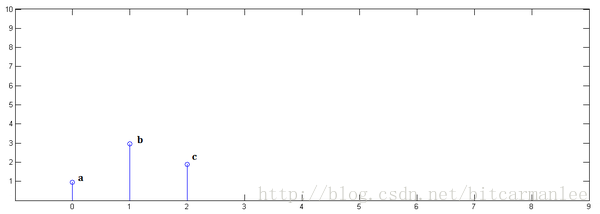
\includegraphics[width=0.9\textwidth]{图像及其数学与物理背景/Figures/卷积x}
\end{figure}

已知$y[0] = i, y[1] = j, y[2] = k$
\begin{figure}[hpbt]
  \centering
  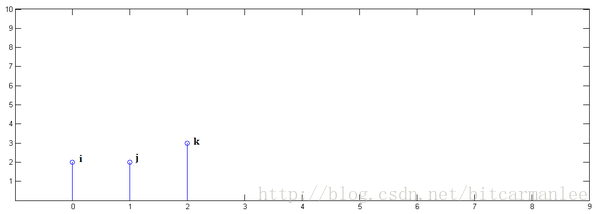
\includegraphics[width=0.9\textwidth]{图像及其数学与物理背景/Figures/卷积y}
\end{figure}

下面通过演示求$x[n] * y[n]$的过程,揭示卷积的物理意义。

第一步,$x[n]$乘以$y[0]$并平移到位置0:
\begin{figure}[hpbt]
  \centering
  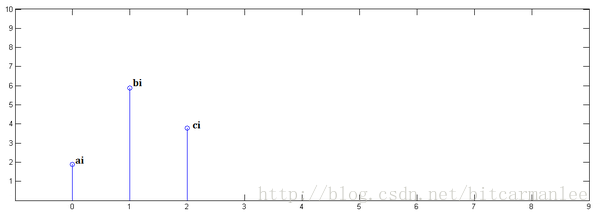
\includegraphics[width=0.9\textwidth]{图像及其数学与物理背景/Figures/卷积1}
\end{figure}

第二步,$x[n]$乘以$y[1]$并平移到位置1 
\begin{figure}[hpbt]
  \centering
  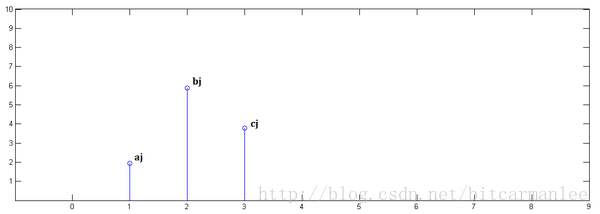
\includegraphics[width=0.9\textwidth]{图像及其数学与物理背景/Figures/卷积2}
\end{figure}

第三步,$x[n]$乘以$y[2]$并平移到位置2 
\begin{figure}[hpbt]
  \centering
  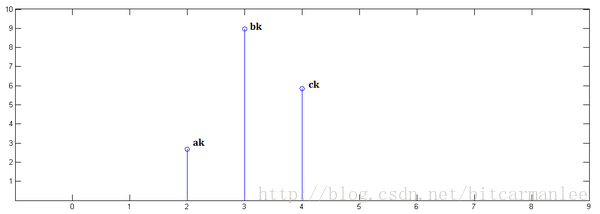
\includegraphics[width=0.9\textwidth]{图像及其数学与物理背景/Figures/卷积3}
\end{figure}

最后,把上面三个图叠加,就得到了$x[n] * y[n]$:
\begin{figure}[hpbt]
  \centering
  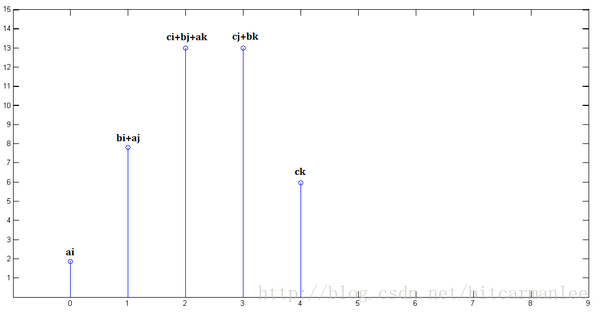
\includegraphics[width=0.9\textwidth]{图像及其数学与物理背景/Figures/卷积4}
\end{figure}

简单吧?无非是平移(没有反褶!)、叠加。%
从这里,可以看到卷积的重要的物理意义是:%
一个函数(如:单位响应)在另一个函数(如:输入信号)上的加权叠加。%
重复一遍,这就是卷积的意义:加权叠加。%


对于线性时不变系统,%
如果知道该系统的单位响应,%
那么将单位响应和输入信号求卷积,%
就相当于把输入信号的各个时间点的单位响应加权叠加,%
就直接得到了输出信号。

通俗的说:%
在输入信号的每个位置,%
叠加一个单位响应,就得到了输出信号。%
这正是单位响应是如此重要的原因。%

在输入信号的每个位置,%
叠加一个单位响应,就得到了输出信号。%
这正是单位响应是如此重要的原因。%

在输入信号的每个位置,%
叠加一个单位响应,就得到了输出信号。%
这正是单位响应是如此重要的原因。%

以上是知乎上排名最高的回答。比较简单易懂。%

\subsection{卷积的另外解释}
卷积表示为$y(n)=x(n)*h(n)$,%
使用离散数列来理解卷积会更形象一点,%
我们把$y(n)$的序列表示成$y(0),y(1),y(2),\cdots$,%
这是系统响应出来的信号。%

同理,$x(n)$的对应时刻的序列为$x(0),x(1),x(2),\cdots$,%
其实我们如果没有学过信号与系统,%
就常识来讲,%
系统的响应不仅与当前时刻系统的输入有关,%
也跟之前若干时刻的输入有关,%
因为我们可以理解为这是之前时刻的输入信号经过一种过程%
(这种过程可以是递减,削弱,或其他)对现在时刻系统输出的影响,%
那么显然,%
我们计算系统输出时就必须考虑现在时刻的信号输入的响应以及之前%
若干时刻信号输入的响应之“残留”影响的一个叠加效果。%
假设0时刻系统响应为$y(0)$,%
若其在1时刻时,此种响应未改变,%
则1时刻的响应就变成了$y(0)+y(1)$,%
叫序列的累加和(与序列的和不一样)。%
但常常系统中不是这样的,%
因为0时刻的响应不太可能在1时刻仍旧未变化,%
那么怎么表述这种变化呢,%
就通过$h(t)$这个响应函数与$x(0)$相乘来表述,%
表述为$x(m)×h(m−n)$,%
具体表达式不用多管,%
只要记着有大概这种关系,%
引入这个函数就能够表述$y(0)$在1时刻究竟削弱了多少,%
然后削弱后的值才是$y(0)$在1时刻的真实值,%
再通过累加和运算,%
才得到真实的系统响应。%

再拓展点,%
某时刻的系统响应往往不一定是由当前时刻和前一时刻这两个响应决定的,%
也可能是再加上前前时刻,%
前前前时刻,前前前前时刻,等等,%
那么怎么约束这个范围呢,%
就是通过对$h(n)$这个函数在表达式中变化后的$h(m−n)$中的$m$的范围来约束的。%
即说白了,就是当前时刻的系统响应与多少个之前时刻的响应的“残留影响”有关。%
当考虑这些因素后,%
就可以描述成一个系统响应了,%
而这些因素通过一个表达式(卷积)即描述出来不得不说是数学的巧妙和迷人之处了。%

\subsection{卷积的应用}
用一个模板和一幅图像进行卷积,%
对于图像上的一个点,%
让模板的原点和该点重合,%
然后模板上的点和图像上对应的点相乘,%
然后各点的积相加,%
就得到了该点的卷积值。%
对图像上的每个点都这样处理。%
由于大多数模板都是对称的,所以模板不旋转。%
卷积是一种积分运算,用来求两个曲线重叠区域面积。%
可以看作加权求和,可以用来消除噪声、特征增强。

把一个点的像素值用它周围的点的像素值的加权平均代替。%
卷积是一种线性运算,%
图像处理中常见的mask运算都是卷积,%
广泛应用于图像滤波。%

卷积关系最重要的一种情况,%
就是在信号与线性系统或数字信号处理中的卷积定理。%
利用该定理,%
可以将时间域或空间域中的卷积运算等价为频率域的相乘运算,%
从而利用FFT等快速算法,%
实现有效的计算,节省运算代价。%

\subsection{补充}
另外在知乎上看到非常好也非常生动形象的解释,特意复制粘贴过来。(知乎马同学的解释)

从数学上讲,卷积就是一种运算。

\noindent{}某种运算,能被定义出来,至少有以下特征:
\begin{enumerate}
\item{首先是抽象的、符号化的}
\item{其次,在生活、科研中,有着广泛的作用}
\end{enumerate}

\noindent{}比如加法:
\begin{enumerate}
\item{a+b,是抽象的,本身只是一个数学符号}
\item{在现实中,有非常多的意义,比如增加、合成、旋转等等}
\end{enumerate}

卷积,是我们学习高等数学之后,新接触的一种运算,%
因为涉及到积分、级数,所以看起来觉得很复杂。%
\begin{figure}[hpbt]
  \centering
  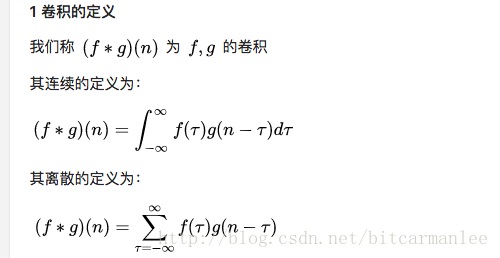
\includegraphics[width=0.9\textwidth]{图像及其数学与物理背景/Figures/原理1}
\end{figure}

这两个式子有一个共同的特征: 
\begin{figure}[hpbt]
  \centering
  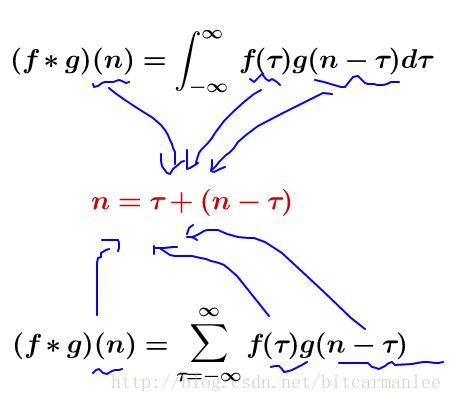
\includegraphics[width=0.6\textwidth]{图像及其数学与物理背景/Figures/原理2}
\end{figure}

这个特征有什么意义?

只看数学符号,卷积是抽象的,不好理解的,%
但是,我们可以通过现实中的意义,%
来习惯卷积这种运算,正如我们小学的时候,%
学习加减乘除需要各种苹果、糖果来帮助我们习惯一样。

我们来看看现实中,这样的定义有什么意义。

离散卷积的例子:丢骰子
\noindent{}我有两枚骰子:
\begin{figure}[hpbt]
  \centering
  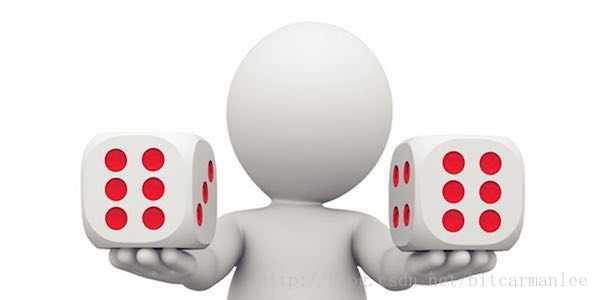
\includegraphics[width=0.6\textwidth]{图像及其数学与物理背景/Figures/色子1}
\end{figure}
把这两枚骰子都抛出去: %
求:两枚骰子点数加起来为4的概率是多少?%
这里问题的关键是,两个骰子加起来要等于4,这正是卷积的应用场景。%

我们把骰子各个点数出现的概率表示出来:
\begin{figure}[hpbt]
  \centering
  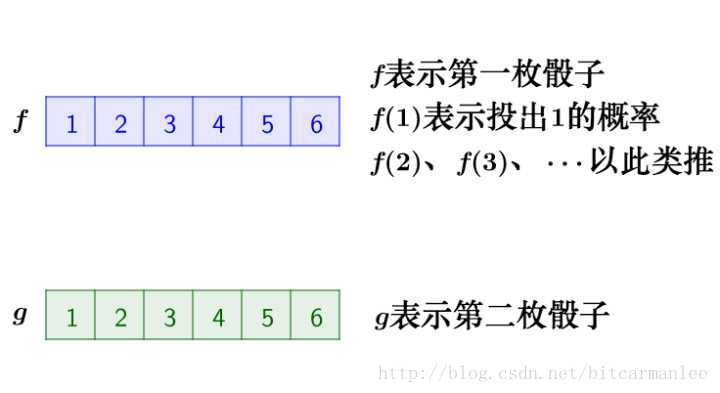
\includegraphics[width=0.6\textwidth]{图像及其数学与物理背景/Figures/色子2}
\end{figure}

那么,两枚骰子点数加起来为4的情况有:
\begin{figure}[hpbt]
  \centering
  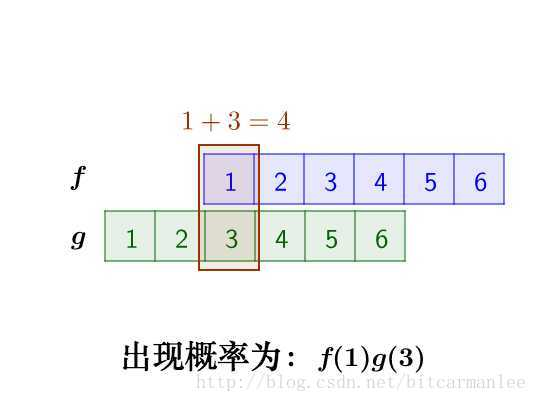
\includegraphics[width=0.6\textwidth]{图像及其数学与物理背景/Figures/色子3}
\end{figure}

\begin{figure}[hpbt]
  \centering
  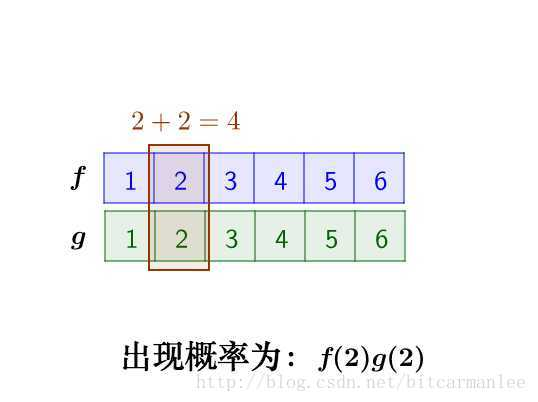
\includegraphics[width=0.6\textwidth]{图像及其数学与物理背景/Figures/色子4}
\end{figure}

\begin{figure}[hpbt]
  \centering
  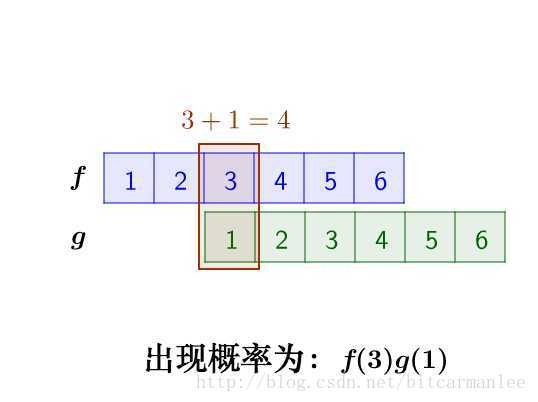
\includegraphics[width=0.6\textwidth]{图像及其数学与物理背景/Figures/色子5}
\end{figure}

因此,两枚骰子点数加起来为4的概率为:
\begin{equation}
  f(1)g(3)+f(2)g(2)+f(3)g(1)
\end{equation}

符合卷积的定义,把它写成标准的形式就是:
\begin{equation}
  (f*g)(4) = \sum_{m=1}^{3}f(4-m)g(m)
\end{equation}

\subsection{连续卷积的例子:做馒头}
连续卷积的例子:做馒头

楼下早点铺子生意太好了,%
供不应求,就买了一台机器,不断的生产馒头。%
假设馒头的生产速度是$f(t)$,%
那么一天后生产出来的馒头总量为:%
\begin{equation}
  \int_{0}^{24}f(t)dt
\end{equation}

馒头生产出来之后,就会慢慢腐败,%
假设腐败函数为$g(t)$,%
比如,10个馒头,24小时会腐败:%
$10*g(t)$
想想就知道,第一个小时生产出来的馒头,%
一天后会经历24小时的腐败,%
第二个小时生产出来的馒头,%
一天后会经历23小时的腐败。%
如此,我们可以知道,%
一天后,馒头总共腐败了:%
\begin{equation}
  \int_{0}^{24}f(t)g(24-t)dt
\end{equation}
这就是连续的卷积。

\subsection{图像处理 }
\subsubsection{原理}
有这么一副图像,可以看到,图像上有很多噪点:
\begin{figure}[hpbt]
  \centering
  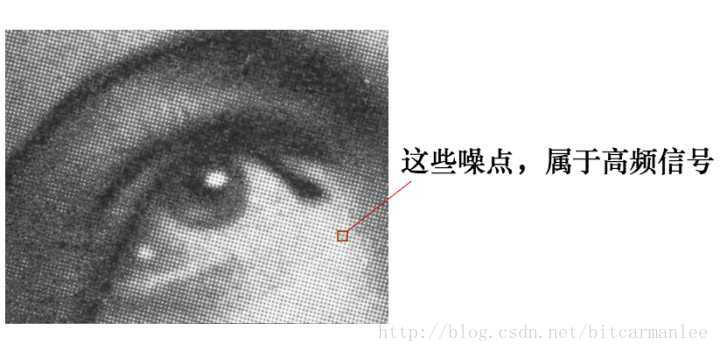
\includegraphics[width=0.6\textwidth]{图像及其数学与物理背景/Figures/图像卷积原理1}
\end{figure}

高频信号,就好像平地耸立的山峰:
\begin{figure}[hpbt]
  \centering
  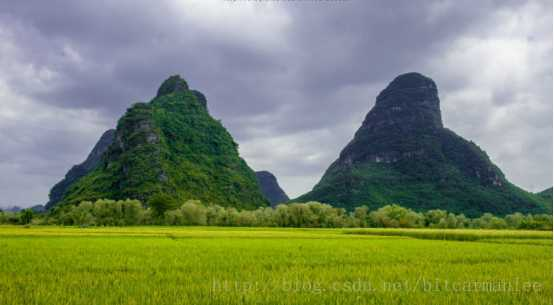
\includegraphics[width=0.6\textwidth]{图像及其数学与物理背景/Figures/图像卷积原理2}
\end{figure}

看起来很显眼。%
平滑这座山峰的办法之一就是,%
把山峰刨掉一些土,填到山峰周围去。%
用数学的话来说,就是把山峰周围的高度平均一下。%
平滑后得到: %
\begin{figure}[hpbt]
  \centering
  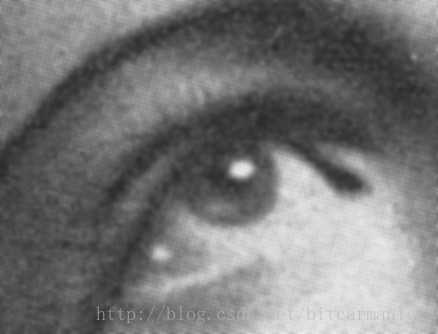
\includegraphics[width=0.4\textwidth]{图像及其数学与物理背景/Figures/图像卷积原理3}
\end{figure}

卷积可以帮助实现这个平滑算法。%
有噪点的原图,可以把它转为一个矩阵: 
\begin{figure}[hpbt]
  \centering
  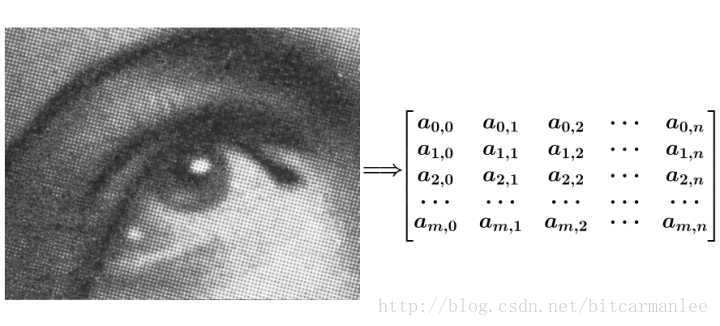
\includegraphics[width=0.8\textwidth]{图像及其数学与物理背景/Figures/图像卷积原理4}
\end{figure}

然后用下面这个平均矩阵(说明下,%
原图的处理实际上用的是正态分布矩阵,%
这里为了简单,%
就用了算术平均矩阵)%
来平滑图像:
\begin{gather}
  g = 
  \begin{bmatrix}
    \frac{1}{9} & \frac{1}{9} & \frac{1}{9} \\
    \frac{1}{9} & \frac{1}{9} & \frac{1}{9} \\
    \frac{1}{9} & \frac{1}{9} & \frac{1}{9} \\
  \end{bmatrix}
\end{gather}

记得刚才说过的算法,%
把高频信号与周围的数值平均一下就可以平滑山峰。%

比如我要平滑$a_{1,1}$点,%
就在矩阵中,取出$a_{1,1}$点附近的点组成矩阵$f$,%
和$g$进行卷积计算后,再填回去
\begin{figure}[hpbt]
  \centering
  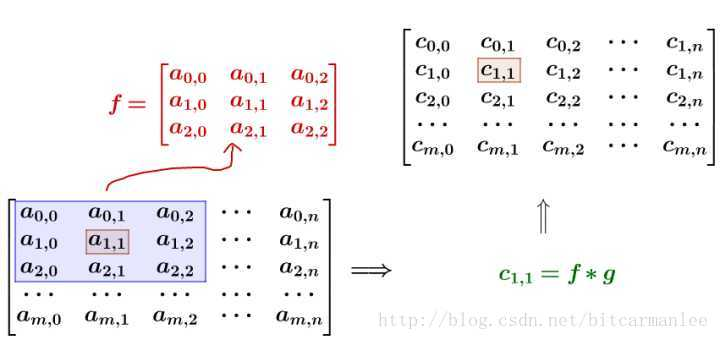
\includegraphics[width=\textwidth]{图像及其数学与物理背景/Figures/图像卷积原理5}
\end{figure}

要注意一点,为了运用卷积,%
$g$虽然和$f$同维度,%
但下标有点不一样:
\begin{figure}[hpbt]
  \centering
  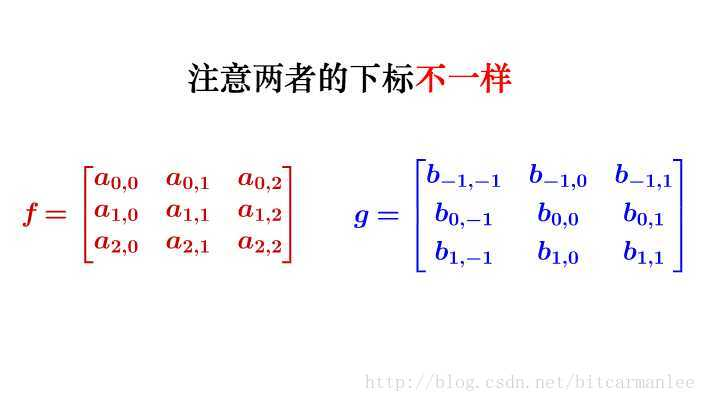
\includegraphics[width=0.8\textwidth]{图像及其数学与物理背景/Figures/图像卷积原理6}
\end{figure}

\begin{figure}[hpbt]
  \centering
  \includegraphics[width=0.8\textwidth]{图像及其数学与物理背景/Figures/图像卷积原理7}
\end{figure}

写成卷积公式就是:
\begin{equation}
  (f*g)(1,1) = \sum_{k=0}^{2}\sum_{h=0}^{2}f(h,k)g(1-h,1-k)
\end{equation}
要求其它的$c_{4,5}$,%
一样可以套用上面的公式.
这样相当于实现了$g$这个矩阵在原来图像上的划动%
(准确来说,下面这幅图把$g$矩阵旋转了$\pi$角度).%




















%%% Local Variables:
%%% mode: latex
%%% TeX-master: t
%%% End:
